\documentclass[coursework]{SCWorks}

\usepackage{preamble}

% Стандартные настройки оформления кода для C++ и Python
\setminted[python]{
    frame=lines,
    framesep=2mm,
    baselinestretch=1.2,
    fontsize=\footnotesize,
    linenos,
    breaklines=true
}
\setminted[cpp]{
    frame=lines,
    framesep=2mm,
    baselinestretch=1.2,
    fontsize=\footnotesize,
    linenos,
    breaklines=true
}

% Красивая нумерация строк в minted
\renewcommand\theFancyVerbLine{\footnotesize\arabic{FancyVerbLine}}

% Русская подпись для окружения listing из minted
\renewcommand{\listingscaption}{Листинг}

\begin{document}

% Кафедра (в родительном падеже)
\chair{математической кибернетики и компьютерных наук}

% Тема работы
\title{Алгоритм Евклида и его реализация на языке Python}

% Курс
\course{1}

% Группа
\group{151}

% Направление
\napravlenie{09.03.04 "--- Программная инженерия}

% Фамилия, имя, отчество в родительном падеже
\author{Шкурата Артёма Сергеевича}

% Заведующий кафедрой
\chtitle{доцент, к.\,ф.-м.\,н.}
\chname{С.\,В.\,Миронов}

% Научный руководитель
\satitle{доцент, к.\,ф.-м.\,н.}
\saname{Г.\,Г.\,Наркайтис}

% Год выполнения отчёта
\date{2026}

\maketitle

% Нумерация рисунков, формул и таблиц по разделам
\secNumbering

\tableofcontents

\intro

Алгоритм Евклида "--- один из старейших известных алгоритмов, применяемый для
нахождения наибольшего общего делителя (НОД) двух целых чисел. Несмотря на
свою простоту, алгоритм имеет фундаментальное значение в теории чисел и
криптографии и до сих пор широко используется на практике~\cite{knuth1997art}.

В настоящей работе кратко описывается математическая основа алгоритма,
приводится его реализация на языке Python и обсуждается асимптотика числа
итераций.

\section{Математическое описание алгоритма}

\textbf{Наибольший общий делитель} двух целых чисел $a$ и $b$, не равных
одновременно нулю, "--- это наибольшее положительное число $d$, на которое
делятся и $a$, и $b$ без остатка~\cite{cormen2013algorithms}. Обозначается
он как $\gcd(a, b)$.

Алгоритм Евклида опирается на следующее свойство НОД:
\begin{equation}\label{eq:recurrence}
    \gcd(a, b) = \gcd(b, a \bmod b), \quad b \neq 0.
\end{equation}

Базовый случай рекурсии "--- когда второй аргумент становится равным нулю:
\begin{equation}\label{eq:base}
    \gcd(a, 0) = a.
\end{equation}

Применяя соотношение~\eqref{eq:recurrence} многократно, можно за конечное
число шагов прийти к базовому случаю~\eqref{eq:base}, поскольку
последовательность остатков строго убывает.

НОД связан с наименьшим общим кратным (НОК) известным тождеством:
\begin{equation}\label{eq:gcd-lcm}
    \mathrm{lcm}(a, b) = \dfrac{|a \cdot b|}{\gcd(a, b)}.
\end{equation}

Это позволяет вычислять НОК через НОД, не реализуя для него отдельный
алгоритм.

\section{Реализация на языке Python}

В листинге~\ref{code:euclid} приведена реализация алгоритма Евклида на
языке Python. Функция \mintinline{python}{gcd_recursive} реализует
рекурсивный вариант, а \mintinline{python}{gcd_iterative} "--- итеративный.
Аргументы \texttt{a} и \texttt{b} "--- неотрицательные целые числа.

\begin{listing}[H]
\inputminted{python}{code/euclid.py}
\caption{Реализация алгоритма Евклида на языке Python}
\label{code:euclid}
\end{listing}

Итеративная версия предпочтительнее с практической точки зрения: она не
тратит память на стек вызовов и обычно работает чуть быстрее. Однако
рекурсивная запись ближе к исходной математической формулировке~%
\eqref{eq:recurrence} и проще читается. Подробное обсуждение разных
вариантов алгоритма можно найти в~\cite{eMaxx-euclid}.

\section{Анализ числа итераций}

Согласно теореме Ламе, число шагов алгоритма Евклида для входных чисел
$a, b \leqslant n$ не превосходит $\log_\varphi(n + 1)$, где
$\varphi = (1 + \sqrt{5}) / 2$ "--- золотое сечение~\cite{knuth1997art}.
Наихудший случай достигается на парах соседних чисел Фибоначчи.

На рисунке~\ref{fig:flowchart} приведена блок"=схема итеративной версии
алгоритма. На рисунке~\ref{fig:iterations} показано, как растёт число
итераций с увеличением входных данных: среднее значение и максимум по
случайной выборке хорошо согласуются с теоретической оценкой Ламе.

\begin{figure}[H]
    \centering
    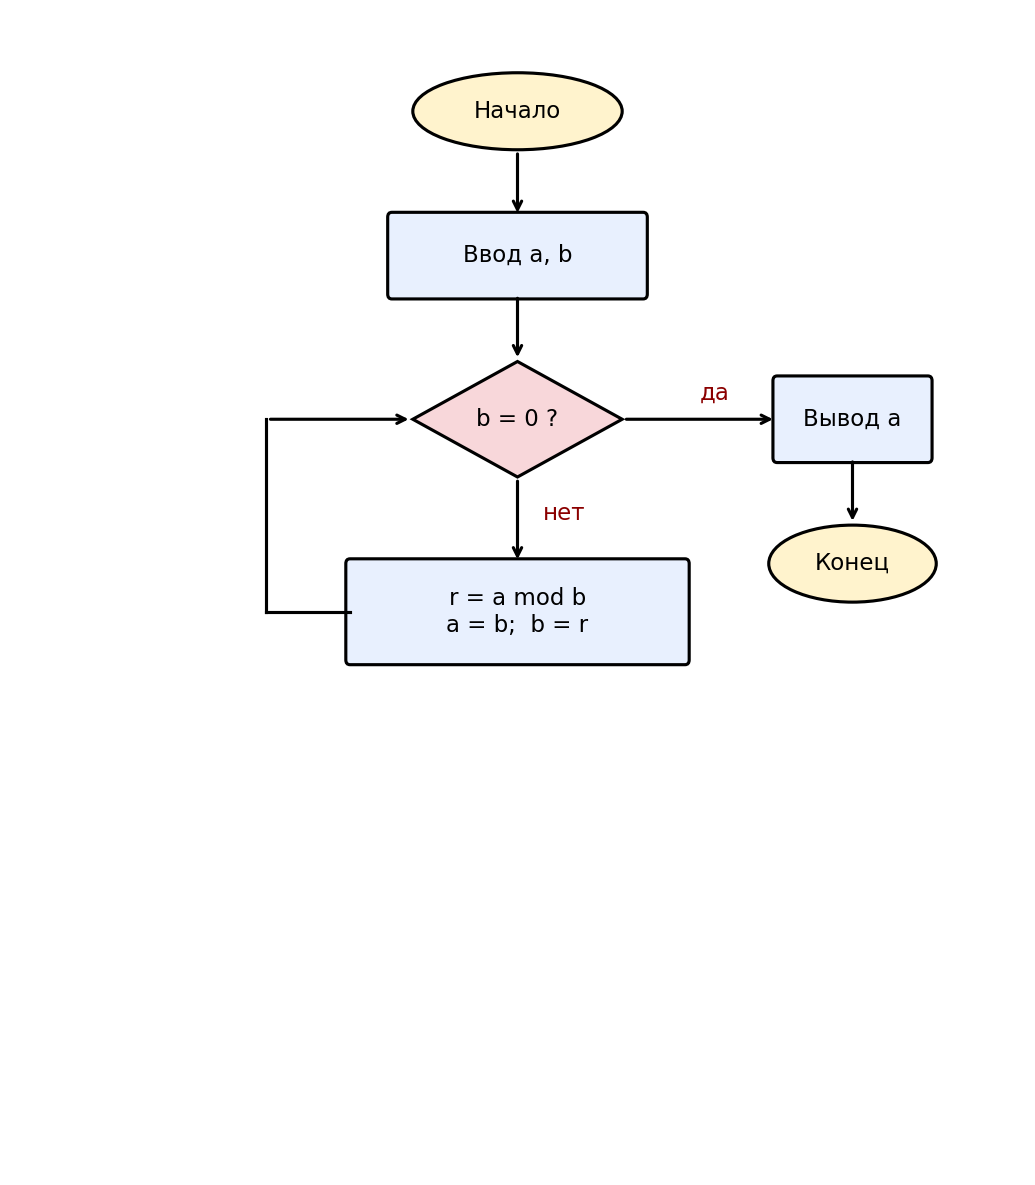
\includegraphics[width=0.55\textwidth]{images/flowchart.png}
    \caption{Блок"=схема алгоритма Евклида}
    \label{fig:flowchart}
\end{figure}

\begin{figure}[H]
    \centering
    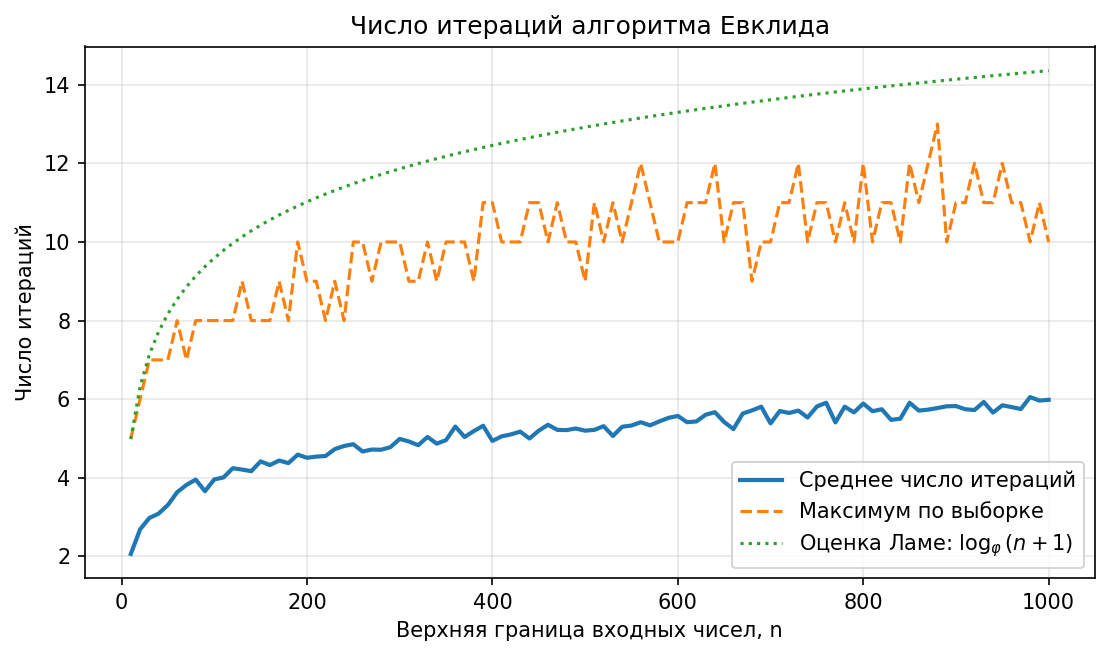
\includegraphics[width=0.95\textwidth]{images/iterations.png}
    \caption{Число итераций алгоритма Евклида в зависимости от размера входа}
    \label{fig:iterations}
\end{figure}

Для нескольких конкретных пар входных чисел в таблице~\ref{tab:examples}
приведены значения НОД и число итераций, выполненных итеративной версией
алгоритма.

\begin{table}[H]
    \centering
    \caption{Примеры работы алгоритма Евклида}
    \label{tab:examples}
    \begin{tabular}{|c|c|c|c|}
        \hline
        $a$ & $b$ & $\gcd(a, b)$ & Число итераций \\
        \hline
        48     & 18    & 6  & 3 \\
        \hline
        1071   & 462   & 21 & 4 \\
        \hline
        100    & 75    & 25 & 2 \\
        \hline
        144    & 89    & 1  & 10 \\
        \hline
    \end{tabular}
\end{table}

Последняя строка таблицы~\ref{tab:examples} соответствует двум соседним
числам Фибоначчи "--- именно на таких парах алгоритм работает наиболее
медленно.

\conclusion

В работе рассмотрен алгоритм Евклида для нахождения НОД, приведены его
математическое обоснование и реализация на языке Python. Анализ числа
итераций показал, что алгоритм обладает логарифмической сложностью и
вполне практичен даже для больших входных чисел.

\bibliographystyle{ugost2003}
\bibliography{thesis}

\end{document}
